
\chapter{HARDroid: Reconocedor de Actividades Humanas}

\label{chap5:hardroid}

\section{Introducción}

\label{sec51:intro}En este capítulo introducimos un sistema que clasifica
las actividades humanas ambulatorias utilizando teléfonos móviles
inteligentes con la plataforma \emph{\abbr{Android}\texttrademark}:
\emph{\abbr{HARDroid}}. El sistema es una adaptación del diseño utilizado
por sistemas existentes como \emph{Google Play Services} \cite{Google2013l},
específicamente la funcionalidad para reconocer actividades humanas
utilizando los conceptos y técnicas expuestos en capítulos precedentes. 

El sistema \emph{\abbr{HARDroid}} está implementado en base a dos
componentes principales: una interfaz de programación que expone las
facilidades y un servicio en ejecución que realiza las funciones principales
del sistema. La interfaz para programadores (\emph{Application Programming
Interface}, \abbr{API}) proporciona una firma de funciones bien definidas
junto con la documentación adecuada para que toda aplicación móvil
de terceros utilice como un componente externo la solución de un sistema
\abbr{HAR}. El servicio de la plataforma \emph{\abbr{Android}} es
una aplicación de segundo plano para teléfonos móviles que implementa
algoritmos de reconocimiento de actividades humanas.

La propuesta de este trabajo se basa en un diseño desacoplado para
contar con una implementación genérica y extensible de un sistema
\abbr{HAR}. Como en todo sistema de \emph{software}, el diseño adecuado
posibilita la evolución y mantenimiento del mismo sin afectar el funcionamiento
de otras aplicaciones móviles clientes dependientes. 

Las siguientes secciones se encuentran organizadas como sigue: primeramente
en la sección \ref{sec52:dise=0000F1o} damos una introducción de
las consideraciones de diseño y metodología utilizadas para la construcción
de los componentes de software. Se empieza con los conceptos generales
de Ingeniería de Software hasta concluir con los detalles técnicos
de la plataforma \emph{\abbr{Android}}. La siguiente sección \ref{sec53:arquitectura}
incluye una vista general del sistema explicando su arquitectura.
La sección \ref{sec54:hardroid} conforma el núcleo principal de este
proyecto donde una implementación \abbr{HAR} en forma de aplicación
móvil desacoplada es presentada. También, en la sección \ref{sec55:activity}
se explica el desenvolvimiento de una herramienta para realizar experimentos
y evaluar los resultados asociados a la solución. Por último, en la
sección \ref{sec56:conclusion} se discuten los resultados preliminares
obtenidos como motivo de los componentes de software construidos.

\section{Diseño General}

\label{sec52:dise=0000F1o}La construcción del sistema \emph{\abbr{HARDroid}
}está enmarcado dentro del ecosistema de aplicaciones móviles. Desde
el punto de vista conceptual del desarrollo de aplicaciones móviles
es necesario enfocarse en dos aspectos principales para el diseño:
el medio y el contexto.

Una aplicación móvil puede presentarse en diversos medios que corresponden
con el enfoque técnico \cite{Fling2009}, es decir: un sitio Web Móvil,
una aplicación Web Móvil, \abbr{SMS}, Juegos, controles utilitarios\footnote{\emph{Widgets}}
y aplicaciones nativas. Las aplicaciones nativas son uno de los medios
más utilizados debido a la rica experiencia de usuario y capacidades
que pueden ser explotadas en los dispositivos, ya que disponen de
gran soporte en la plataforma subyacente. Por ejemplo, en la plataforma
para teléfonos móviles \emph{\abbr{Android} }se dispone de capacidades
tales como almacenamiento, ubicación, acceso a los sensores del dispositivo
y además de un medio de distribución certificado como ser \emph{Google
Play Store} \cite{Google2016p}. 

Por otro lado, está el contexto de la aplicación que se refiere a
la experiencia que el usuario final obtiene al utilizar el sistema
móvil. Para esto el sistema móvil procesa la información de contexto
que rodea al usuario dándose una interacción distinta a los sistemas
convencionales. A continuación, se listan los tipos de contexto comunes
utilizados en las aplicaciones móviles y un breve ejemplo de su funcionalidad
\cite{Fling2009}:
\begin{itemize}
\item \emph{Utilidad}: Calculadora, Conversión de monedas.
\item \emph{Localización}: Mapas, Registro de actividades físicas.
\item \emph{Informativo}: Buscar información relevante.
\item \emph{Productividad}: Comprar productos y pagar servicios
\item \emph{Inmersión}: Juegos 
\end{itemize}
Estos tipos de contexto se pueden combinar para crear mejores experiencias
de uso de la aplicación móvil. El trabajo desarrollado en esta tesis
se adecua al modelo de aplicaciones móviles de contexto. Se busca
proveer un componente de \emph{Utilidad} que puede ser combinado con
diferentes aplicaciones móviles desarrolladas por terceros y pueda
ser mantenidas en forma colaborativa. 

\subsection{Criterios de Diseño}

\label{ssec52:criterios-dise=0000F1o}La implementación de este trabajo,
así como la mayoría de los sistemas de información, se rige bajo el
principio de diseño \emph{basado en componentes} donde se busca separar
la complejidad de un sistema en módulos y que estos interactúen entre
sí. Los módulos en el diseño de sistemas mejoran la flexibilidad y
comprensión mientras se reduce el tiempo de desarrollo de los mismos
\cite{Parnas1972}.

Una de las técnicas más comunes de diseño de sistemas\emph{ }es la
separación por capas (\emph{Layering)} para dividir un sistema complejo
\cite{Fowler2002} en diferentes niveles. 

\subsubsection{Arquitecturas en Capas}

Cuando un sistema se construye en términos de capas, los módulos se
organizan en niveles apilados como en un pastel, donde cada capa se
soporta sobre las capas inferiores. En este sentido, la capa superior
utiliza varios servicios definidos en capas inferiores, pero la capa
inferior desconoce y no depende de las capas en niveles superiores.
Las capas definen concretamente las responsabilidades y encapsulan
las funcionalidades soportadas en cada nivel.

La popularidad de la división de sistemas en módulos por capas se
volvió más relevante con el auge de los sistemas tipo \emph{Cliente-Servidor}.
Estos sistemas fueron inicialmente concebidos como de dos capas: el
cliente se encarga de la interfaz de usuario y la lógica de la aplicación,
y el servidor usualmente es una base de datos relacionales. En la
\figref{fig5:cliente_servidor} se muestra una representación de la
arquitectura en dos capas. Para sistemas sencillos que desplieguen
información y actualicen datos, este modelo es el más adecuado. Sin
embargo, a medida que se construyen sistemas más complejos, el problema
radica mantener la lógica central del sistema: las reglas de negocio,
validaciones, cálculos, etc. El modelo de dos capas propone ubicar
la lógica central embebida en las interacciones de la Interfaz de
Usuario, la capa cliente, o almacenar los mismos en procedimientos
almacenados en la basa de datos, la capa servidor.

\begin{figure}[H]
\begin{centering}
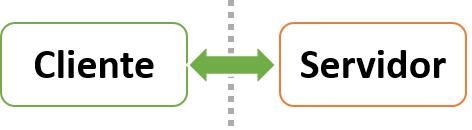
\includegraphics[width=0.6\columnwidth]{capitulo-5/graphics/cliente_servidor}
\par\end{centering}
\caption[Modelo de dos capas]{\label{fig5:cliente_servidor}Modelo de dos capas}
\end{figure}

Debido a las limitaciones del enfoque Cliente-Servidor, se puede extender
el mismo con la ayuda del paradigma de Orientación a Objetos para
construir sistemas con arquitecturas de tres capas. Estas capas son
comúnmente conocidas como \cite{Fowler2002}: Presentación, Dominio
y Recursos. En la \tabref{tab5:tres_capas} se definen las responsabilidades
correspondientes a cada capa. 

\begin{table}[H]
\begin{centering}
\begin{tabular}[t]{|l|>{\raggedright}p{0.5\columnwidth}|}
\hline 
Capa & Responsabilidades\tabularnewline
\hline 
\hline 
Presentación & Provisión de servicios a sistemas externos, despliegue de información
e interacción con el usuario.\tabularnewline
\hline 
Dominio & \multirow{1}{0.5\columnwidth}{Lógica y procesamiento del sistema.}\tabularnewline
\hline 
Recursos & Comunicación con bases de datos, sistemas externos, integración, transacciones
y otros componentes.\tabularnewline
\hline 
\end{tabular}
\par\end{centering}
\caption[Modelo de tres capas]{\label{tab5:tres_capas}Modelo de tres capas}
\end{table}

Independientemente del tipo de sistema de información a ser construido,
al dividir el mismo en capas lógicas o dividir el sistema en partes
separadas se permite reducir el acoplamiento entre diferentes módulos,
inclusive si todos los módulos se ejecutan en la misma máquina física.
En la \figref{fig5:tres_capas} se muestra la arquitectura de tres
capas discutida anteriormente.

\begin{figure}[H]
\begin{centering}
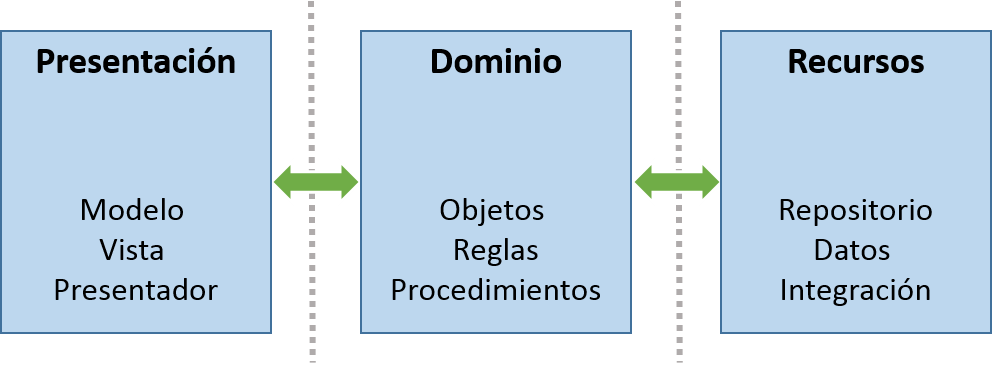
\includegraphics[width=0.8\columnwidth]{capitulo-5/graphics/arqui_tres_capas}
\par\end{centering}
\caption[Modelo de tres capas]{\label{fig5:tres_capas}Modelo de tres capas}

\end{figure}


\subsubsection{Patrones de Diseño}

Los patrones de diseño son un concepto importante del paradigma de
orientación a objetos, que han sido ideados para solucionar problemas
comunes determinados en un contexto particular \cite{Shalloway2004}.
Una definición acertada es la que se cita a continuación.
\begin{quotation}
<<\emph{Cada patrón describe un problema que ocurre una y otra vez
en nuestro entorno, y también describe la solución principal al problema,
de tal manera que la solución pueda ser utilizada millares de veces,
sin tener que duplicar el trabajo de pensar cómo resolver el problema.>>}
\cite{Alexander1977}
\end{quotation}
Para nuestro objetivo de diseño se utilizan los siguientes patrones
de diseño para organizar la capa de \emph{Dominio} cuya responsabilidad
es la lógica principal del sistema. Se sigue la técnica de dividir
la capa de\emph{ Dominio} por medio de los siguientes patrones \cite{Fowler2002}:
\begin{enumerate}
\item \emph{Service Layer}: Capa de servicios
\item \emph{Domain Model}: Modelo del dominio
\end{enumerate}
La capa de servicios es el punto de interacción entre la \emph{Presentación}
y el\emph{ Dominio}, por lo que actúa como proveedor de una interfaz
clara (comúnmente una \abbr{API} de programación). Este patrón define
los límites del sistema con una capa de servicios que establece el
conjunto de operaciones disponibles y coordina el proceso de cada
operación. La capa de servicios puede ser tan gruesa o tan fina como
se requiera, puede contener objetos de servicio con reglas de negocio,
manejo de transacciones, seguridad, entre otros.

Por otro lado, el modelo del dominio da soporte a la capa de servicios.
Este patrón define objetos de dominio que tienen incorporados datos
y comportamientos, estos representan de manera significativa el dominio
del problema a resolver. Debido a que la lógica de negocio de un sistema
puede ser bastante compleja, estos objetos están diseñados para manejar
las diversas combinaciones de reglas y lógica del sistema.

\subsubsection{Guías Generales}

En este trabajo fueron utilizadas las guías generales para construcción
de sistemas orientados a objetos. Algunos de los principios más relevantes
que han sido considerados durante el diseño de nuestra solución son
\cite{Albin2003}:
\begin{itemize}
\item Modularidad
\item Orientación a Objetos
\item Reusabilidad
\item Ocultamiento de Información
\item Abstracción
\end{itemize}
Siguiendo estos principios se ha logrado una implementación exitosa
de los componentes y aplicaciones móviles clientes de verificación.
Además, se ha enfocado el desarrollo con miras a la colaboración basada
en la comunidad de código abierto por medio de una Licencia Pública
Apache, Versión 2.0 (\emph{Apache License Version 2.0}, en inglés)
\cite{GimenezYegros2016c}.

\subsection{Metodología de Desarrollo}

\label{ssec52:metodologia}En toda labor de construcción de sistemas
de información es necesario definir una metodología de diseño para
encarar problemas y tecnologías complejas. La metodología utilizada
en este trabajo es el diseño descendente (\emph{top-down desing}),
que permite organizar el diseño del sistema en niveles de abstracción
para reducir la complejidad general del sistema \cite{Albin2003}. 

En esta metodología se empieza definiendo la funcionalidad esperada
del sistema como lo requiere el cliente, la capa más alta, y sigue
paso a paso hasta refinar el diseño en capas más bajas a medida que
se avanzan con detalles específicos. 

El diseño empieza poniendo énfasis en las funcionalidades esperadas
del sistema cuando este se encuentre en operación. Luego, se continúa
con el diseño de la lógica de negocios que soportan a estas funcionalidades,
y por último se enfoca en los recursos necesarios por la capa lógica.

Como aspecto práctico de esta metodología se han identificado las
siguientes tareas específicas de diseño que ayudan a comprender y
describir mejor el desarrollo de este trabajo:
\begin{enumerate}
\item Diseñar la arquitectura de la solución.
\item Diseñar la capa de servicios, o interfaz del sistema enfocada para
programadores (\abbr{API}) con un conjunto de llamadas a exponer.
\item Diseño de los recursos que conforman el dominio al servicio.
\item Implementación del servicio reconocedor.
\item Implementación de un componente de evaluación de la solución.
\end{enumerate}
Parte de la metodología consistió en definir la interfaz del sistema
en base a las mejores prácticas de la industria para aplicaciones
móviles de contexto, utilizando el lenguaje de programación \emph{\abbr{Java}}
y la tecnología basada en \emph{\abbr{Android}}. El diseño se basa
en implementaciones existentes \cite{Google2016m} para heredar las
buenas prácticas de programación y obtener la ventaja de familiaridad
de la \abbr{API} para desarrolladores.

\subsection{Tecnología}

\label{ssec52:tecnologia}Esta sección está dedicada a describir la
tecnología utilizada para la implementación del diseño de este trabajo.
Uno de los criterios claves para la selección de teléfonos móviles
inteligentes apropiados para el reconocimiento de actividades, además
de los sensores, es el sistema operativo (\emph{Operating System},
\abbr{OS}) móvil. 

El sistema operativo móvil se encarga del manejo de recursos del dispositivo
y el control de operación de las aplicaciones móviles. Estos sistemas
tienen características similares a los sistemas operativos convencionales
utilizados en las computadoras de escritorio (\emph{Personal Computer},
\abbr{PC}). La función principal de un sistema operativo es proveer
servicios comunes a las aplicaciones y administrar los recursos de
\emph{hardware}. Adicionalmente, los sistemas operativos móviles están
diseñados para el uso eficiente de energía, debido a las limitaciones
de batería, y características especiales de movilidad. 

En este trabajo se propone una herramienta que está dirigida a los
teléfonos móviles inteligentes basados en \emph{\abbr{Android}}.
En los siguientes apartados se da una vista general de \emph{\abbr{Android}
}como plataforma tecnológica de este capítulo.

\subsubsection{Plataforma}

El sistema operativo móvil \emph{\abbr{Android}} es una plataforma
de código abierto con un entorno de programación de distribución publica,
que además incluye una interfaz de programación (\abbr{API}) completa
con acceso al \emph{hardware} del teléfono y los sensores internos.
Esta facilidad permite que las herramientas de aprendizaje automático
y sus procedimientos puedan ser construidos de manera más simple. 

\emph{\abbr{Android}} es una plataforma abierta para dispositivos
móviles encabezada por \emph{Google} y la \emph{Open Handset Alliance
\cite{OHA2008}} con el objetivo de innovar en el entorno móvil, mejorando
la experiencia de usuario a un menor costo \cite{Gargenta2014}. El
principal aporte que logró \emph{\abbr{Android}} es que por primera
vez una plataforma abierta consigue separar el \emph{software} y el
\emph{hardware} subyacente. Esto permite que un gran número diverso
de dispositivos ejecuten las mismas aplicaciones, creando un ecosistema
más variado para desarrolladores y consumidores. 

\subsubsection{Arquitectura}

La plataforma \emph{\abbr{Android}} está soportada sobre el núcleo
(\emph{\abbr{Kernel}}) de\emph{ \abbr{Linux} }cuyo proyecto al igual
es una iniciativa de código abierto utilizado ampliamente en el ámbito
de tecnología de la información desde hace más de una década. La capa
más baja de la arquitectura hereda las principales funcionalidades
esperadas en los sistemas operativos modernos: portabilidad, seguridad
y las capacidades funcionales.

\begin{figure}[H]
\begin{centering}
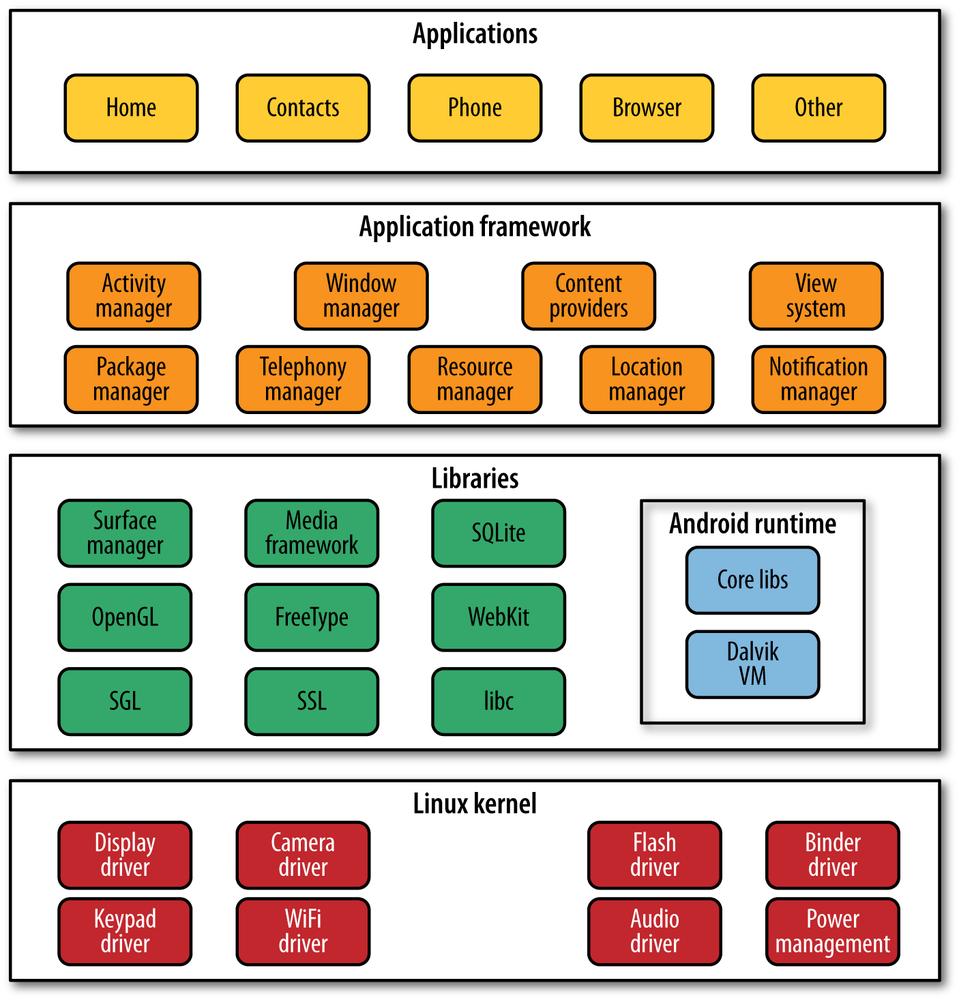
\includegraphics[width=0.7\columnwidth]{capitulo-5/graphics/android_stack}
\par\end{centering}
\caption[Arquitectura de Android]{\label{fig5:android-stack}Arquitectura de \abbr{Android}}
\end{figure}

Adicionalmente, la plataforma ha mejorado el núcleo introduciendo
un número de extensiones especiales para el entorno móvil. Las extensiones
agregan capacidades funcionales mejoradas para administrar la energía;
ya que los móviles utilizan batería, mecanismos para llamados a procedimientos
remotos y aislamiento para mejorar la seguridad \cite{Gargenta2014}.
Las extensiones fueron módulos agregados cuya lista se detalla a continuación
con su nomenclatura en inglés \cite{Schreiber2011}: 
\begin{itemize}
\item \emph{Alarm }
\item \emph{Ashmem}
\item \emph{Binder}
\item \emph{Power Management}
\item \emph{Low Memory Killer}
\item \emph{Kernel debugger} y \emph{Kernel} \emph{logger}
\end{itemize}
En la \figref{fig5:android-stack} se muestra la plataforma \emph{\abbr{Android}}
con todos los componentes que están soportados sobre el núcleo y que
en la siguiente sección se detallan.

\subsubsection{Componentes}

Los componentes de la plataforma mostrados en la \figref{fig5:android-stack}
se agrupan en las siguientes partes \cite{Gargenta2014} (con nomenclatura
inglesa):
\begin{itemize}
\item \textbf{Native Layer}: Este componente llamado capa nativa es un conjunto
base de funcionalidades implementadas en \texttt{C/C++} que no forman
parte del núcleo sino del espacio de usuario del sistema. Este grupo
está compuesto de varias partes como: abstracciones de \emph{hardware}
(\emph{Hardware Abstraction Layer}, \abbr{HAL}), librerías nativas,
servicios del sistema y herramientas básicas utilitarias.
\item \textbf{Dalvik}: Es una máquina virtual (\emph{Dalvik Virtual Machine},
\abbr{DVM}) de propósito específico diseñada especialmente para \emph{\abbr{Android}}
de manera que este corra aplicaciones programadas en el lenguaje \emph{\abbr{Java}}
\cite{Ehringer2010}. A diferencia de la máquina virtual de Java estándar
(\emph{Java Virtual Machine}, \abbr{JVM}), el diseño se hizo pensando
en restricciones específicas de los entornos móviles, como consumo
de energía y capacidad limitada de recursos como \abbr{CPU} y Memoria.
Además, la \abbr{JVM} posee restricciones de licencia comercial.
\item \textbf{Application Framework}: Este componente provee un entorno
de programación con varias librerías y servicios para construir aplicaciones
nativas. Este componente es el que está mejor documentado y cubierto
en toda la plataforma ya que permite a los desarrolladores ser creativos
y construir aplicaciones que puedan ser distribuirlas al mercado.
Son parte de este componente las librerías \emph{\abbr{Java} }genéricas
y las específicas de \emph{\abbr{Android}} \cite{Android2016r},
como también servicios (o gestores de recursos) que facilitan las
capacidades útiles de la plataforma como ubicación, sensores, conectividad,
etc. 
\item \textbf{Applications}: Las aplicaciones son el punto de acceso principal
de la plataforma y se soporta sobre los componentes arriba mencionados.
La función principal de la aplicación es proveer una utilidad al usuario
final según lo descrito inicialmente en la sección \ref{sec52:dise=0000F1o}.
Las aplicaciones pueden estar instaladas de fábrica en los teléfonos
móviles o pueden ser adquiridos por los usuarios en los mercados de
distribución de aplicaciones\emph{ \abbr{Android}}.
\end{itemize}

\subsection{Marco de Trabajo}

\label{ssec52:framework}En esta sección, se exponen las facilidades
de \emph{\abbr{Android}} como marco de trabajo (\emph{framework}),
es decir, desde el punto de vista del entorno de programación que
ofrece, con énfasis en las características disponibles para crear
aplicaciones contextuales. Este apartado presenta una vista de alto
nivel acerca de los modelos de computación y comunicación disponibles
en la plataforma.

\subsubsection{Componentes de Computación}

Los bloques principales de una aplicación móvil son componentes que
\emph{\abbr{Android}} provee para construir una aplicación contextual
de utilidad. La idea de este apartado es presentar a grandes rasgos
los componentes disponibles y como estos se combinan entre sí para
formar una aplicación. Cada aplicación está compuesta de cuatro (4)
componentes distintos, donde cada uno cubre un tópico en específico
\cite{Gargenta2014}. Los componentes son descritos a continuación
(con nomenclatura inglesa):
\begin{itemize}
\item \textbf{\emph{Activity}}: El componente \emph{actividad} representa
la interfaz de usuario de la aplicación responsable de desplegar la
información y capturar las interacciones. Este componente no persiste
información, sino que son tareas de cómputo de corta duración y en
primer plano donde el sistema operativo puede requerir pararlos y
pasarlos a un modo de reposo frecuentemente.
\item \textbf{\emph{Service}}: El componente \emph{servicio} ofrece un mecanismo
para ejecutar tareas de computo de larga duración en segundo plano
sin interfaz de usuario asociada. Un servicio solo puede ser parado
si el sistema se queda sin recursos de memoria.
\item \textbf{\emph{Content Provider}}: El componente \emph{proveedor} de
contenido provee una interfaz para compartir datos entre aplicaciones.
Su función es la persistencia de datos por medio de una \abbr{API}
que sigue el principio \abbr{CRUD} (\emph{Create, Read, Update and
Delete}), una forma de acceso parecida al de las bases de datos \abbr{SQL}.
Los datos pueden ser persistidos en archivos locales o recursos remotos
en red.
\item \textbf{\emph{Broadcast Receiver}}: El componente \emph{receptor}
de mensajes provee un mecanismo para publicación y suscripción a eventos
del sistema basado en el patrón de diseño \emph{Observer} \cite{Shalloway2004}.
El receptor ejecuta una tarea de computo latente que se activa con
la ocurrencia de un evento para lo cual está suscrito. Los eventos
tienen la forma de mensajes que es descrito en la siguiente sección.
\end{itemize}
Estos componentes en su conjunto conforman una aplicación móvil. Estos
son bloques básicos que están conectados de manera suelta y están
contenidos en un entorno de aplicación que comparten un proceso del
sistema operativo y compiten por los mismos recursos: memoria, archivos,
\abbr{CPU}, etc.

\subsubsection{Componente de Comunicación}

El intercambio de datos es una necesidad común entre componentes de
un sistema (o entre sistemas diferentes). En \emph{\abbr{Android}},
el intercambio es realizado por medio de un mecanismo denominado \emph{Inter-Process
Communication} (\abbr{IPC}): una comunicación entre procesos, o comunicación
entre componentes si forman parte de la misma aplicación \cite{Schreiber2011}. 

Cada aplicación dispone de dos (2) componentes que resuelven un tópico
en particular y son descritos a continuación (con nomenclatura inglesa):
\begin{itemize}
\item \textbf{\emph{Intent}}: El componente \emph{mensaje} es una representación
de las operaciones a ser realizadas. Consiste en una estructura de
datos que contiene un identificador en formato \abbr{URI}, una acción
asociada y datos anexos que son procesados por el sistema de comunicación
entre procesos. 
\item \textbf{\emph{IPC Binder}}: El componente \emph{procesador} que implementa
el mecanismo de comunicación entre procesos \emph{\cite{Schreiber2011}}
y se discute con más detalle durante el desenvolvimiento de este trabajo\emph{.
}El sistema operativo\emph{ \abbr{Android}} junto con su marco de
trabajo operan como un sistema distribuido y la tecnología para lograr
su diseño se basa completamente en este componente.
\end{itemize}
En la \figref{fig5:mensajes-ipc} se muestran las diferentes formas
de interacción entre los componentes \emph{\abbr{Android} }citados
anteriormente. Como se puede apreciar, todas las interacciones son
llevadas a cabo por el mecanismo principal de llamadas \abbr{IPC}.

Una actividad se inicia por medio de un mensaje y puede lanzar otra
actividad en pantalla. Un servicio se inicia, se para y se asocia
por el mecanismo \abbr{IPC} como también las llamadas a métodos y
retorno de resultados son realizados por el mismo medio. Un proveedor
de contenidos es consultado con llamadas \abbr{IPC} y retorna los
resultados por el mismo medio. Todos los eventos son recibidos por
el receptor de mensajes por medio del \abbr{IPC}. Como es manifiesto
en la gráfica, el marco de trabajo de \emph{IPC Binder} se basa el
modelo \emph{Cliente-Servidor} (ver \ref{ssec52:criterios-dise=0000F1o})
y el patrón de diseño \emph{Proxy} \cite{Shalloway2004}.

\begin{figure}[H]
\begin{centering}
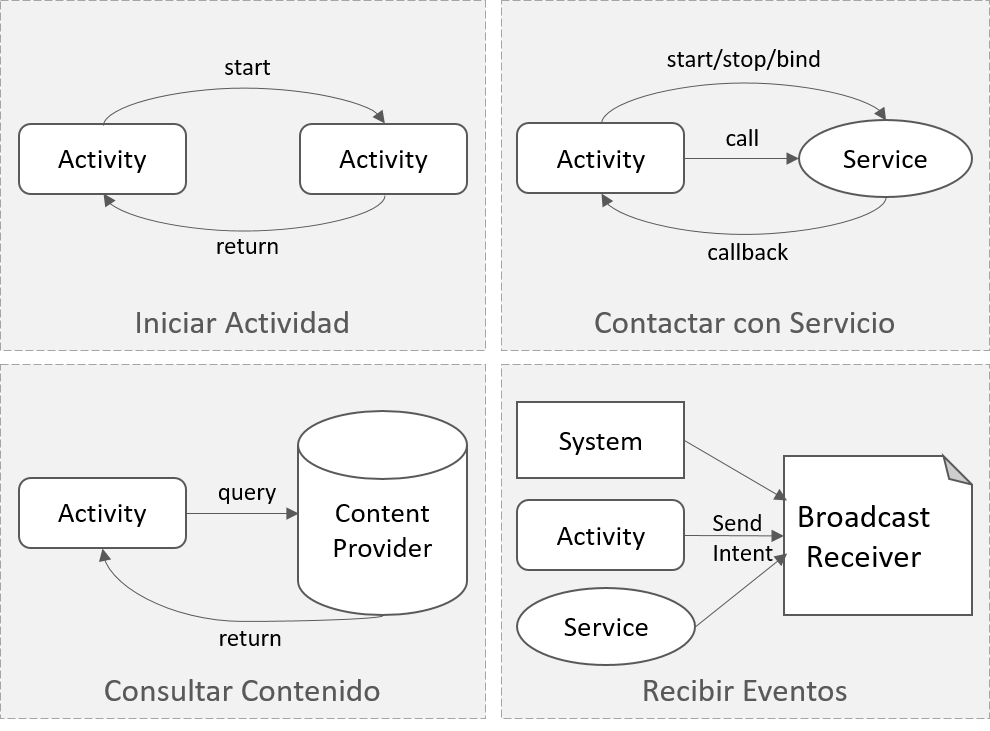
\includegraphics[width=1\columnwidth]{capitulo-5/graphics/mensajes_ipc}
\par\end{centering}
\caption[\emph{Framework Android}]{\label{fig5:mensajes-ipc}Marco de Trabajo \abbr{Android}}
\end{figure}


\section{Arquitectura del Proyecto}

\label{sec53:arquitectura}La solución presentada en este trabajo
puede describirse partiendo el mismo en tres componentes principales:
\begin{itemize}
\item \textbf{\emph{HARDroid}}: Es un servicio de reconocimiento de actividades
humanas específico para \emph{\abbr{Android}}. Este componente tiene
cabida dentro de la capa de \emph{Application Framework} descrita
en \ref{ssec52:tecnologia} como un servicio utilitario. El algoritmo
reconocedor de actividades es un componente dinámico capaz de actualizar
su clasificador continuamente.
\item \textbf{\emph{ActivitySurvey}}: Es una aplicación móvil de encuesta
que permite utilizar el servicio de reconocimiento y además evaluar
el resultado con el consentimiento del usuario. Este componente está
ubicado en la capa de \emph{Applications} descrita en \ref{ssec52:tecnologia}.
El resultado evaluado puede ser utilizado para mejorar el clasificador
de aprendizaje automático.
\item \textbf{\emph{Backend C4.5}}: Es un servicio web basado en el estilo
\emph{Representational State Transfer} (\abbr{REST}) que recolecta
evaluaciones del usuario que utiliza la aplicación de encuesta. Además,
almacena los resultados que surgen debido a la utilización del reconocedor
con el objetivo de crear el modelo de aprendizaje automático de manera
manual. 
\end{itemize}
\begin{figure}[H]
\begin{centering}
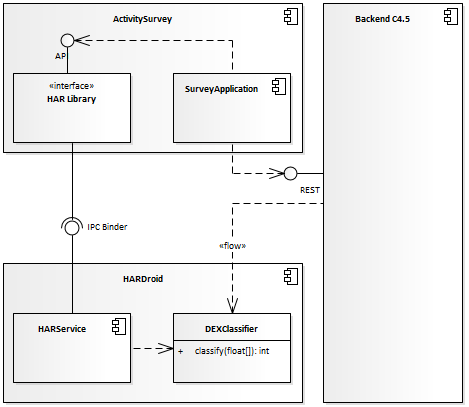
\includegraphics[width=1\columnwidth]{capitulo-5/graphics/arqui_general}
\par\end{centering}
\caption[Arquitectura del Proyecto]{\label{fig5:arqui-general}Arquitectura del Proyecto}

\end{figure}

En la \figref{fig5:arqui-general} se ilustra la vista general de
la arquitectura del proyecto donde se muestran los dos aportes principales
de este trabajo junto con sus partes relevantes, que son \emph{HARDroid}
y \emph{ActivitySurvey} \cite{GimenezYegros2016b}. El diagrama se
describe en lenguaje \abbr{UML} donde los componentes representan
las aplicaciones móviles distribuidas de manera independiente y un
componente de servidor (es decir que no se ejecuta dentro de los dispositivos
móviles, sino que está disponible a los mismos desde la nube) para
recolectar datos experimentales, siendo este último el componente
\emph{Backend C4.5}.

\section{HARDroid: Servicio de Reconocimiento}

\label{sec54:hardroid}El servicio \emph{\abbr{HARDroid} }fue diseñado
para ajustarse a las características generales de los gestores y/o
servicios en la capa de \emph{Application Framework} de \emph{\abbr{Android}},
Ej. \emph{Location Manager} o \emph{Google Play Services}. La ventaja
del servicio \emph{\abbr{HARDroid}} para las aplicaciones móviles
hechas por terceros es que aprovechan las últimas mejoras del motor
de reconocimiento de actividades, con actualización automática de
la plataforma distribuida como un \abbr{APK} independiente a través
de la tienda \emph{Google Play} \cite{GimenezYegros2016a}. Esto permite
a los usuarios estar actualizados y los desarrolladores poseen mecanismos
fáciles para integrarse al servicio \abbr{HAR}.

\begin{figure}[H]
\begin{centering}
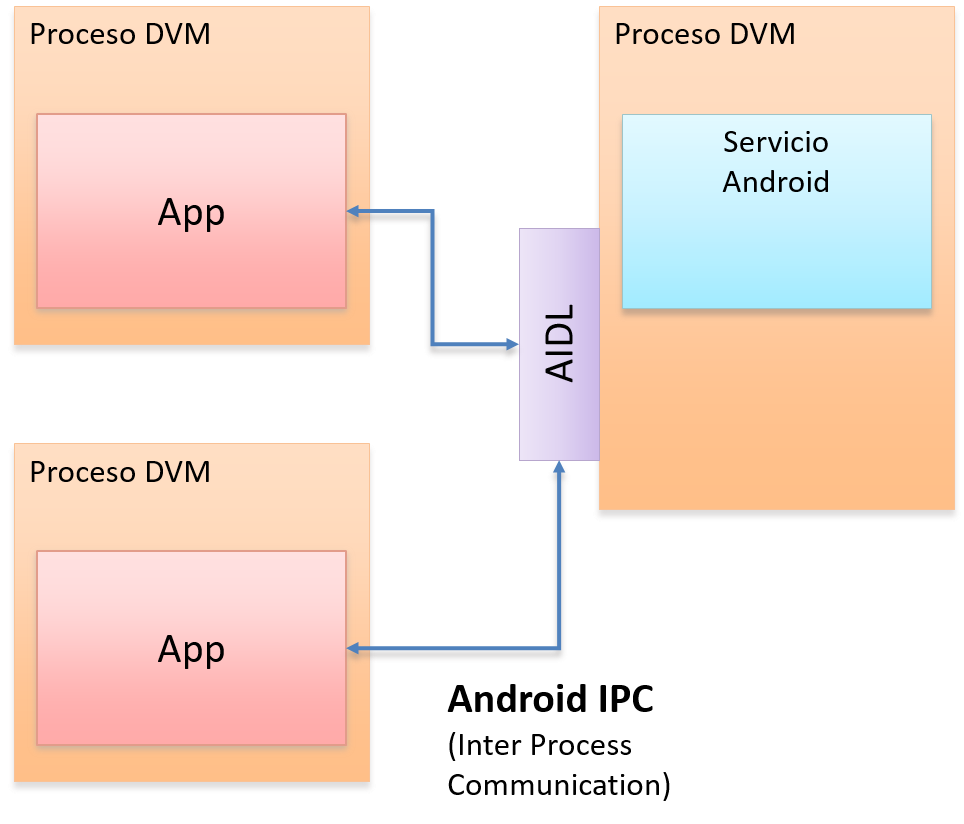
\includegraphics[width=0.7\columnwidth]{capitulo-5/graphics/hardroid_func}
\par\end{centering}
\caption[Servicio HARDroid]{\label{fig5:hardroid-func}Servicio \abbr{HARDroid}}

\end{figure}

En la \figref{fig5:hardroid-func} se muestra el esquema de funcionamiento
del servicio \emph{\abbr{HARDroid}} en base al diseño expuesto en
el párrafo anterior. Este esquema de diseño es el más apropiado para
crear aplicaciones móviles distribuidas en \emph{\abbr{Android}},
semejante a la arquitectura de servicios de \emph{Google Play Services}
\cite{Google2016l}. Las aplicaciones móviles están confinadas en
procesos separados del sistema \emph{\abbr{Android}}, cada cual en
su entorno \abbr{DVM} correspondiente, donde la comunicación entre
procesos es llevado a cabo por medio de una interfaz denominada \emph{Android
Interface Definition Language} (\abbr{AIDL}) que forma parte del
mecanismo \emph{IPC Binder} (ver sección \ref{ssec52:framework}).

\subsection{Módulos Funcionales}

\label{ssec54:modulos}Desde el punto de vista conceptual el servicio
\emph{\abbr{HARDroid}} puede ser dividido en cuatro módulos principales
que cumplen con las características específicas que se describen a
continuación.

\subsubsection{Interfaz de Servicio}

Este módulo define el modelo dominio y la interfaz de integración
(a través de una \abbr{API}). En el dominio del problema se identificaron
los siguientes conceptos:
\begin{itemize}
\item \emph{Cliente} (\texttt{\small{}ActivityRecognitionClient}): Un cliente
es un proceso remoto que requiere reconocer actividades humanas con
cierta periodicidad.
\item \emph{Conexión} (\texttt{\small{}ServiceConnection}):\emph{ }Es una
entidad que mantiene la información de estado del servicio como sesión
del cliente. Posee un ciclo de vida de conexión y cierre.
\item \emph{Actividad Humana} (\texttt{\small{}HumanActivity}): Es una entidad
que modela una actividad humana reconocida.
\item \emph{Vector Característico} (\texttt{\small{}Feature}): Es una entidad
que modela el conjunto de valores característicos utilizados durante
el procesamiento de la señal de los sensores.
\item \emph{Resultado de Reconocimiento} (\texttt{\small{}ActivityRecognitionResult}):
Es un conjunto de actividades humanas reconocidas junto con la precisión
estimada y los datos complementarios generados durante el cálculo
en forma de vector característico.
\end{itemize}
En la \figref{fig5:domain-model} se muestra el diagrama de clases
con los artefactos construidos para el manejo del dominio del problema.
Las clases se definieron con semejanza a los conceptos de \emph{Google
Play Services} \cite{Google2016l} y la documentación se detalla en
\cite{GimenezYegros2016d}.

La interfaz del servicio se compone de un conjunto de llamadas para
que cualquier cliente disponga de las siguientes acciones:
\begin{itemize}
\item \emph{Conectarse} al servicio
\item \emph{Desconectarse} del servicio
\item \emph{Suscribirse} con cierta periodicidad a resultados de actividades
humanas detectados. 
\item \emph{Obtener} el resultado de actividades humanas detectado más reciente.
\end{itemize}
\begin{figure}[H]
\begin{centering}
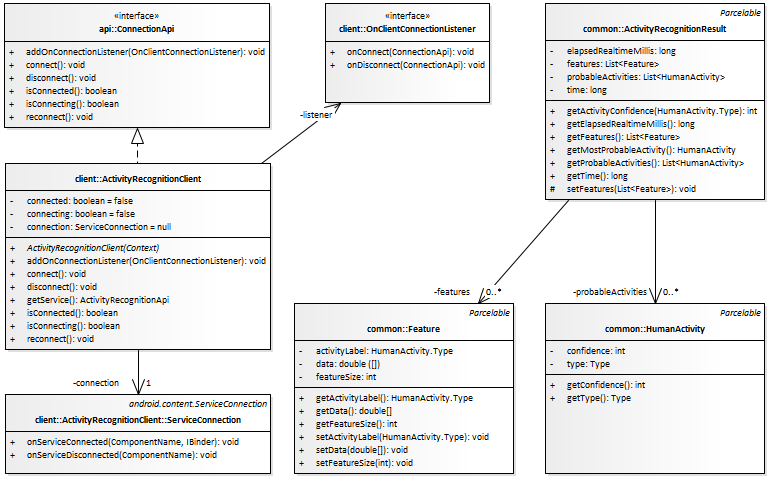
\includegraphics[width=1\columnwidth]{capitulo-5/graphics/class_domain}
\par\end{centering}
\caption[Diagrama de clases del dominio del problema]{\label{fig5:domain-model}Diagrama de clases del dominio del problema.}
\end{figure}

Teniendo en consideración el modelo de dominio y las acciones requeridas
se presenta la interfaz del servicio en el diagrama de clases de la
\figref{fig5:service-layer}.

\begin{figure}[H]
\begin{centering}
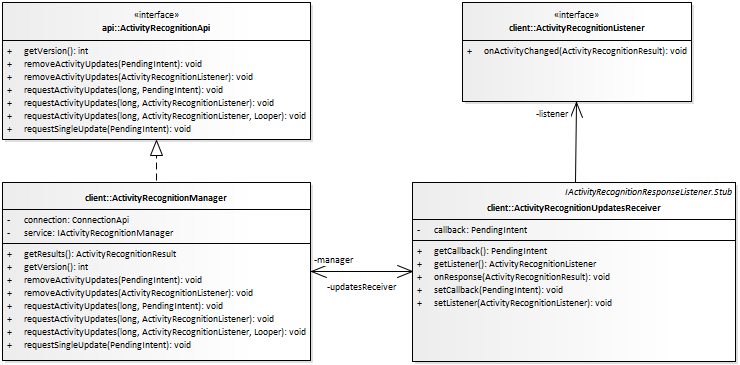
\includegraphics[width=1\columnwidth]{capitulo-5/graphics/class_service}
\par\end{centering}
\caption[Diagrama de clases de la capa de servicio]{\label{fig5:service-layer}Diagrama de clases de la capa de servicio.}

\end{figure}

Para poder clarificar la interfaz proveída por la capa de servicios
se describe textualmente el contrato definido por la \abbr{API} para
suscribirse a eventos de detección actividades humanas:
\begin{itemize}
\item \texttt{\footnotesize{}requestSingleUpdate(callbackIntent: PendingIntent): void
public} \\
Obtiene el resultado de detección de actividad más reciente 
\item \texttt{\footnotesize{}requestActivityUpdates(detectionIntervalMillis: long,
}~\\
\texttt{\footnotesize{}listener: ActivityRecognitionListener): void
public}\\
Se suscribe a eventos de detección de actividad a intervalos regulares
en mili-segundos. Espera la respuesta con un observador.
\item \texttt{\footnotesize{}requestActivityUpdates(detectionIntervalMillis: long,
}~\\
\texttt{\footnotesize{}callbackIntent: PendingIntent): void public}
\\
Se suscribe a eventos de detección de actividad a intervalos regulares
en mili-segundos. Espera la respuesta con una función diferida.
\item \texttt{\footnotesize{}removeActivityUpdates(listener: ActivityRecognitionListener): void
public} \\
Se cancela la subscripción a eventos de detección de actividad teniendo
en cuenta el observador registrado.
\item \texttt{\footnotesize{}removeActivityUpdates(callbackIntent: PendingIntent): void
public}\\
Se cancela la subscripción a eventos de detección de actividad teniendo
en cuenta la función diferida registrada.
\end{itemize}
En las siguientes secciones se detallan los módulos encargados de
implementar la lógica de negocio y las funcionalidades de esta interfaz.

\subsubsection{Servidor}

Este módulo implementa el servidor de llamadas a procedimientos remotos
desde clientes distribuidos en otros procesos. La lógica de negocio
se divide en dos responsabilidades para manejar la conexión y la suscripción
por medio de los siguientes artefactos:
\begin{itemize}
\item \texttt{\small{}ActivityRecognitionService}: Es la función principal
que implementa el servidor \abbr{IPC} de \emph{\abbr{Android} }para
atender las conexiones con los clientes. Además se encarga de registrar
las suscripciones y emitir los resultados de detección de acuerdo
a las preferencias de los clientes. 
\item \texttt{\small{}ActivityRecognitionManagerImpl}: Es un utilitario
que hace de mediador entre las llamadas remotas a la \abbr{API} y
el servidor en ejecución.
\item \texttt{\small{}ActivityRecognitionSubscription}: Es una estructura
de datos para memorizar las preferencias de suscripción de los clientes
administrado por el servidor.
\end{itemize}
La interacción que ocurre durante la conexión de un cliente al servidor
de reconocimiento se muestra en la \figref{fig5:service-subs}. Para
representar la interacción se utiliza un diagrama de secuencia \abbr{UML}
donde las clases en amarillo representan objetos en el proceso del
cliente, a través de la librería cliente \emph{\abbr{HARDroid}}.
Las clases en azul son objetos en el proceso del servidor, a través
de la aplicación móvil \emph{\abbr{HARDroid}}.

\begin{figure}[H]
\begin{centering}
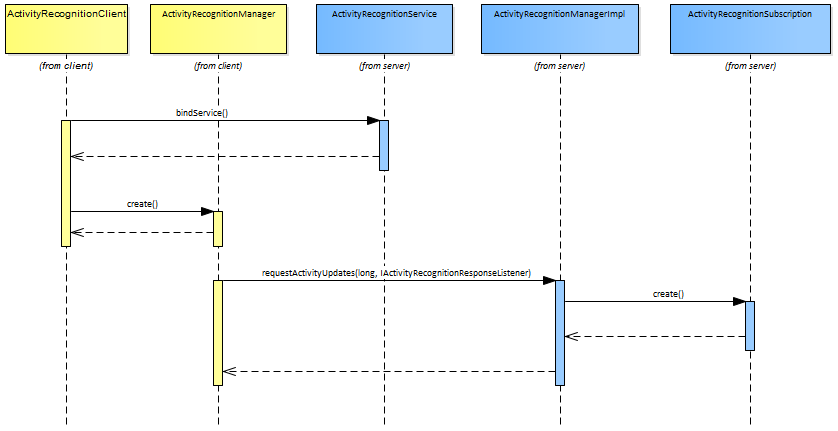
\includegraphics[width=1\columnwidth]{capitulo-5/graphics/service_subs}
\par\end{centering}
\caption[Interacción cliente y servidor de HARDroid]{\label{fig5:service-subs}Interacción cliente y servidor de \abbr{HARDroid}}
\end{figure}

La primeras dos interacciones corresponde a la conexión de clientes
y la tercera interacción es la suscripción. El servidor administra
una lista de suscripciones donde a cada cliente se le registra la
preferencia de notificación ante un evento de actividad detectada. 

\subsubsection{Procesamiento}

Este módulo es el motor de reconocimiento de actividades humanas que
se ejecuta a intervalos periódicos de tiempo siempre que existan suscripciones
registradas. La ejecución del motor produce siempre un resultado global
de actividad humana detectada por medio de los siguientes artefactos: 
\begin{itemize}
\item \texttt{\small{}ActivityRecognitionWorker}: Es la función principal
que ejecuta una tarea periódica de recolección de datos sensoriales,
cálculo de vectores característicos y clasificación de actividad para
producir un nuevo resultado. La producción de un nuevo resultado dispara
un evento de publicación a través del servidor.
\item \texttt{\small{}FeatureProcessing}: Es un utilitario que calcula los
vectores característicos.
\item \texttt{\small{}SignalProcessing}: Es un utilitario con funciones
de procesamiento de señales. 
\end{itemize}
La ejecución del motor de reconocimiento empieza al iniciar el servidor
y se muestra en la \figref{fig5:service-worker}. El motor realiza
las tareas en un intervalo de tiempo definido por el menor tiempo
registrado de acuerdo a las suscripciones de clientes.

\begin{figure}[H]
\begin{centering}
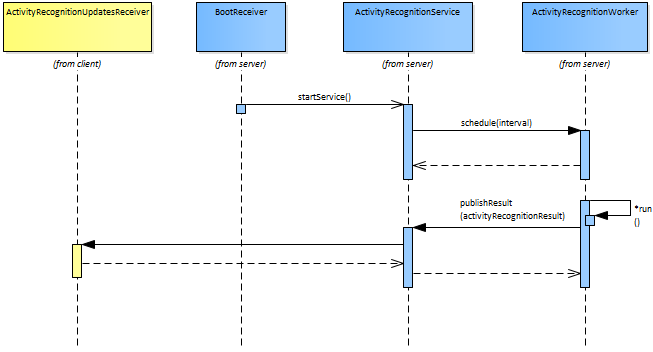
\includegraphics[width=1\columnwidth]{capitulo-5/graphics/service_worker}
\par\end{centering}
\caption[Procesamiento y publicación de resultados de HARDroid]{\label{fig5:service-worker}Procesamiento y publicación de resultados
de \abbr{HARDroid}}
\end{figure}

Ante la eventualidad de un nuevo resultado detectado por el motor
de reconocimiento se realiza una publicación de resultados a los clientes
correspondientes. El algoritmo de reconocimiento se describe a continuación.

\begin{algorithm}[h]
\begin{algorithmic}[1]
    \Require Conjunto de tiempos de subscripción de clientes $S$
	\Procedure{Reconocimiento}{$ S $}
		\If {$S \textit{ está vacío } $}
 			\State\textit{Terminar}
		\EndIf
		\State $t_w \leftarrow 10$
        \Comment{Ventana de tiempo estándar de reconocimiento}
		\State $t_{min} \leftarrow \min_{\forall s \in S} s$
		\State Esperar $t_{min} - t_w$ segundos 
		\State $ a_{xyz} = $ Leer sensor por $t_w$ segundos o 512 muestras
		\State $ C = \emptyset$
		\For{$i := 1 \to 512$}
			\State $ v_f = $ Calcular vector caracteristicos de $a_{xyz}$ con valores entre $[i, i + 127]$
			\State $ c_a = $ Clasificar $v_f$ con el algoritmo \textit{C4.5}
			\State $ C = C \cup \{c_a\}$ 
			\State $i := i + 64$
        \EndFor
        \State $ M = $ Calcular matriz de frecuencia de $C$ 
		\State
		\Return $ M $
	\EndProcedure
\end{algorithmic}

\caption{\label{alg5:reconocimiento}Detección de actividades humanas}
\end{algorithm}


\subsubsection{Clasificador}

Este módulo es responsable de realizar la clasificación de actividades
humanas a partir de un vector característico y produce una estimación
de la actividad humana detectada. Posee dos implementaciones principales
y complementarias de acuerdo a los siguientes artefactos:
\begin{itemize}
\item \texttt{\small{}ActivityClassifier}: Es una clase genérica que define
los métodos comunes para los clasificadores de actividades humanas.
\item \texttt{\small{}DecisionTreeClassifier}: Es la implementación de un
clasificador de actividades humanas basado en arboles de decisión
generados por la herramienta \emph{Waikato Environment Knowledge Analysis}
\texttt{(\abbr{WEKA})} \cite{Frank2016}.
\item \texttt{\small{}DumbClassifier}: Es la implementación de un clasificador
de actividades humanas simple que no produce un resultado válido.
\item \texttt{\small{}DexModelLoader}: Es un utilitario para descargar de
Internet de manera segura un clasificador dinámico generado con \abbr{WEKA}.
El clasificador está implementado en una clase contenida en una librería
de \emph{software} en formato \abbr{JAR}.
\end{itemize}
La actualización dinámica del clasificador se muestra en la \figref{fig5:service-classi}.
Cada nueva versión del clasificador se genera por medio de \abbr{WEKA}
y se construye para luego disponerlo como una librería remota a ser
descargada de Internet. El mecanismo detallado se describe en \cite{Falsina2014}.

\begin{figure}[H]
\begin{centering}
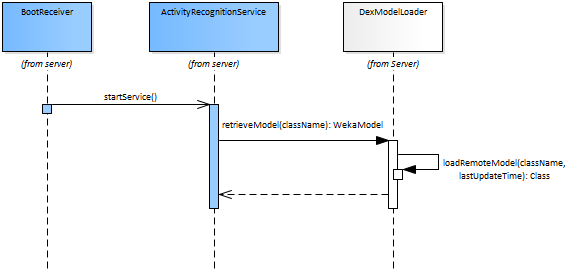
\includegraphics[width=1\columnwidth]{capitulo-5/graphics/service_classi}
\par\end{centering}
\caption[Actualización del clasificador C4.5]{\label{fig5:service-classi}Actualización dinámica del clasificador
C4.5 basado en \abbr{WEKA}}
\end{figure}


\section{ActivitySurvey: Encuesta de Evaluación}

\label{sec55:activity}Con el objetivo de comprobar el funcionamiento
del servicio \emph{\abbr{HARDroid}} desarrollado y evaluar los resultados
producidos al detectar las actividades realizadas por el usuario,
se creó la aplicación \emph{ActivitySurvey \cite{GimenezYegros2016e}.
}El diseño de la aplicación móvil es bastante sencillo pero con los
complementos necesarios que permiten validar las funcionalidades de
\emph{\abbr{HARDroid}} y además encuestar a usuarios reales durante
una sesión de entrenamiento físico. En esta sección se presenta la
vista general de la aplicación explicada por medio de los artefactos
que describen las funcionalidades básicas construidas. 

\subsection{Requerimientos Funcionales}

A continuación se incluyen las especificaciones funcionales que describen
el comportamiento de la aplicación desde el punto de vista del actor
principal: el usuario final. Los asuntos identificados que forman
parte de los requisitos son agrupados en los siguientes puntos.

\subsubsection{Registrarse}

Este requerimiento implica que el usuario accede por primera vez a
la aplicación y debe registrar sus datos personales para poder identificar
a las muestras generadas por una persona en particular. En la siguiente
\figref{fig5:uc-registro} se listan los casos de uso correspondientes.

\begin{figure}[H]
\begin{centering}
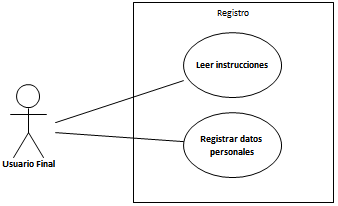
\includegraphics{capitulo-5/graphics/caso_registro}
\par\end{centering}
\caption[Diagrama de Caso de Uso: Registro]{\label{fig5:uc-registro}Diagrama de Caso de Uso: Registro}
\end{figure}

\begin{description}
\item [{CU01-Leer~instrucciones}] El usuario verifica la tarjeta inicial
con notas de bienvenida e instrucciones básicas de uso para luego
accionar el botón <<ENTENDIDO>>. El sistema oculta la tarjeta permanentemente
y dirige a la vista de registro.
\item [{CU02-Registrar~datos~personales}] El usuario visualiza la pantalla
de registro inicial y procede a completar sus datos personales: correo
electrónico, edad e intervalo de detección. El sistema guarda la información
en las preferencias básicas del usuario.
\end{description}

\subsubsection{Responder Encuesta}

Este requerimiento implica la funcionalidad principal de encuesta
donde el usuario debe realizar sesiones de entrenamiento físico que
resultan en registros de señales y la predicción de la actividad física
probable que debe ser aseverada. En la siguiente \figref{fig5:uc-encuesta}
se listan los casos de uso correspondientes.

\begin{figure}[H]
\begin{centering}
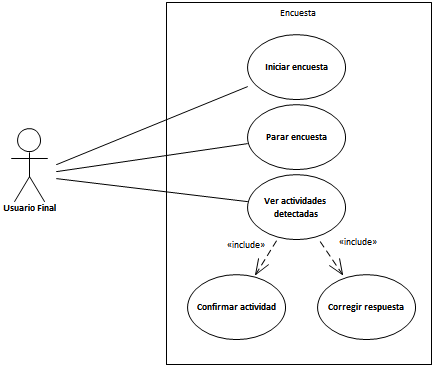
\includegraphics{capitulo-5/graphics/caso_encuesta}
\par\end{centering}
\caption[Diagrama de Caso de Uso: Encuesta]{\label{fig5:uc-encuesta}Diagrama de Caso de Uso: Encuesta}

\end{figure}

\begin{description}
\item [{CU03-Iniciar~Encuesta}] El usuario acciona un botón para iniciar
una nueva sesión de entrenamiento. \\
El sistema se suscribe al servicio de reconocimiento de actividades
teniendo en cuenta las preferencias del usuario y se generan tarjetas
visuales de encuesta periódicamente.
\item [{CU04-Parar~Encuesta}] El usuario acciona un botón para parar la
sesión de entrenamiento activa. \\
El sistema se desconecta del servicio de reconocimiento de actividades.
\item [{CU05-Ver~actividades~detectadas}] El usuario dispone de una lista
de tarjetas visuales de encuesta con los resultados recientes de una
sesión de entrenamiento. 
\item [{CU06-Confirmar~actividad}] El usuario responde positivamente a
la tarjeta visual de encuesta aseverando el resultado de la actividad
humana detectada por medio del botón <<CORRECTO>>. \\
El sistema actualiza la tarjeta de encuesta como detectada correctamente.
\item [{CU07-Corregir~respuesta}] El usuario responde negativamente a
la tarjeta visual de encuesta negando el resultado de la actividad
humana detectada por medio del botón <<INCORRECTO>>. \\
El sistema despliega un dialogo para obtener la actividad humana declarada
por el usuario.\\
El usuario selecciona la actividad humana que corresponde. \\
El sistema actualiza la tarjeta de encuesta con la respuesta del usuario.
\end{description}

\subsubsection{Cambiar Preferencias}

Este requerimiento implica una acción complementaria de cambiar las
preferencias internas que modifican el comportamiento de la aplicación
móvil. En la siguiente \figref{fig5:uc-preferencia} se listan los
casos de uso correspondientes.

\begin{figure}[H]
\begin{centering}
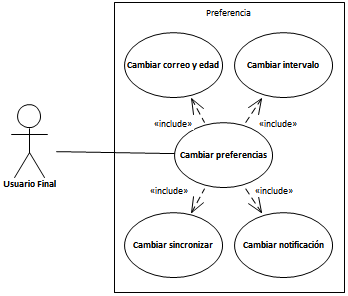
\includegraphics{capitulo-5/graphics/caso_preferencia}
\par\end{centering}
\caption[Diagrama de Caso de Uso: Preferencia]{\label{fig5:uc-preferencia}Diagrama de Caso de Uso: Preferencia}
\end{figure}

\begin{description}
\item [{CU08-Cambiar~preferencias}] El usuario dispone de una lista de
preferencias de edición agrupados por categorías. 
\item [{CU09-Cambiar~correo~y~edad}] El usuario edita sus datos personales:
correo electrónico y edad. \\
El sistema guarda la información en las preferencias del usuario.
\item [{CU10-Cambiar~intervalo}] El usuario edita el intervalo de detección
de actividades. \\
El sistema guarda la información en las preferencias del usuario y
se reinicia la suscripción al servicio de detección de actividades.
\item [{CU11-Cambiar~sincronizar}] El usuario modifica el comportamiento
y el método de sincronizar de datos por red. \\
El sistema guarda la información en las preferencias del usuario y
activa/desactiva sincronizar datos por medio del método seleccionado.
\item [{CU12-Cambiar~notificación}] El usuario modifica el comportamiento
de notificación de nuevas actividades detectadas. \\
El sistema guarda la información en las preferencias del usuario y
activa/desactiva la notificación.
\end{description}

\subsection{Diseño Detallado}

El diseño del proyecto se basa en los componentes comunes de una aplicación
móvil \emph{\abbr{Android} }según lo expuesto en \ref{ssec52:framework}.
El diseño se compone de una colección desacoplada de Actividades,
Servicios, Proveedores y Receptores que se describen a continuación.

\subsubsection{Módulos Funcionales}
\begin{itemize}
\item \texttt{\small{}SurveyApplication}: Es el contexto global de la aplicación
que mantiene acceso a las preferencias, los servicios y las suscripciones
a mensajes.
\item \texttt{\small{}FeedActivity}: Es la vista principal de la aplicación
que despliega la lista de actividades detectadas en una línea de tiempo
como tarjetas de preguntas. Cada pregunta puede ser obviada, corregida
o aseverada. 
\item \texttt{\small{}SettingsActivity}: Es la vista de configuración de
la aplicación que modifica las preferencias del usuario final y las
almacena en el dispositivo móvil.
\item \texttt{\small{}DetectorService}: Es un servicio que mantiene una
conexión persistente con el servicio \emph{\abbr{HARDroid}}. El servicio
es iniciado o parado dependiendo de la necesidad del usuario encuestado.
\item \texttt{\small{}DetectedActivitiesService}: Es un servicio de función
diferida que permite recibir actualizaciones de resultados detectados
por el servicio \emph{HARDroid}. Por cada actividad humana detectada,
persiste la información y notifica por mensaje que existen nuevos
resultados.
\item \texttt{\small{}NotificationReceiver}: Es un receptor de mensajes
para crear alertas auditivas en el momento que se detectan nuevos
resultados. Permite avisar al usuario final que debe contestar una
nueva encuesta.
\item \texttt{\small{}HumanActivityFeed}: Es el proveedor de contenidos
que persiste los resultados a ser evaluados durante la encuesta.
\item \texttt{\small{}UpdateActionReceiver}: Es un receptor de mensajes
que sincroniza los resultados evaluados por los usuarios encuestados
con un servicio remoto.
\end{itemize}
En la \figref{fig5:act-surv-diag} se muestran los módulos funcionales
que hacen a la aplicación con una notación de los componentes de la
plataforma \emph{\abbr{Android} }y su interacción \cite{Gargenta2014}. 

\begin{figure}[H]
\begin{centering}
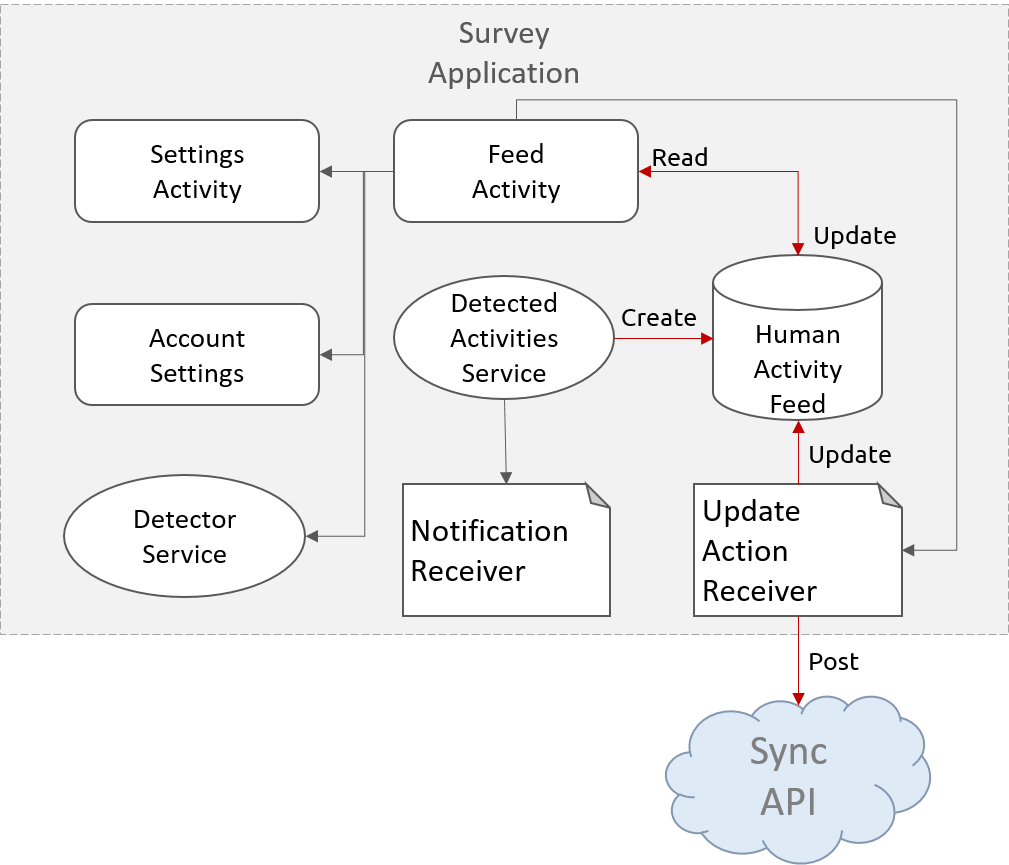
\includegraphics[width=1\columnwidth]{capitulo-5/graphics/act_surv_diag}
\par\end{centering}
\caption[Diagrama de diseño de ActivitySurvey]{\label{fig5:act-surv-diag}Diagrama de diseño de \emph{ActivitySurvey}}

\end{figure}


\subsubsection{Persistencia}

Las actividades humanas detectadas durante una sesión deben ser almacenadas
en el teléfono móvil para luego transmitirlas a un servidor central.
Los resultados de cálculos del reconocedor y las encuestas respondidas
por los usuarios se persisten en una base de datos personal perteneciente
a la aplicación. El diagrama desplegado en la \figref{fig5:act-surv-er}
representa el modelo de datos utilizado. Esta información se sincroniza
por medio un servicio Web externo para un posterior análisis y mejoras
al algoritmo de clasificación.

\begin{figure}[H]
\begin{centering}
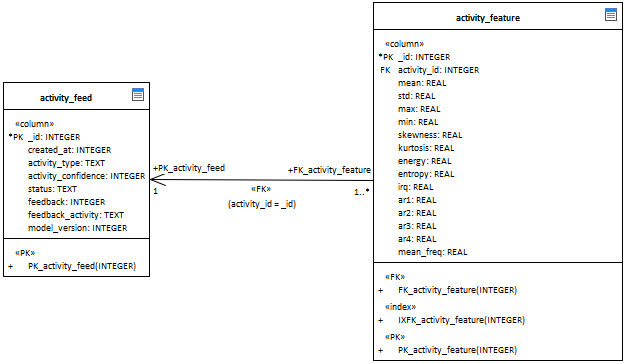
\includegraphics[width=1\columnwidth]{capitulo-5/graphics/act_surv_er}
\par\end{centering}
\caption[Modelo de datos de ActivitySurvey]{\label{fig5:act-surv-er}Modelo de datos de \emph{ActivitySurvey}}
\end{figure}


\subsubsection{Interfaz de Usuario}

En base al modelo de información se presentan los contextos que permiten
a los usuarios navegar y descubrir las vistas y acciones disponibles
en la aplicación móvil. El diagrama de navegación en la \figref{fig5:navega}
muestra la lista completa de pantallas necesarias para que los usuarios
interactúen con los datos. 

En la aplicación de encuesta, los usuarios tienen la capacidad de
ver sus actividades reconocidas, responder a la encuesta confirmando
la actividad o corrigiendo la misma. 

\begin{figure}[H]
\begin{centering}
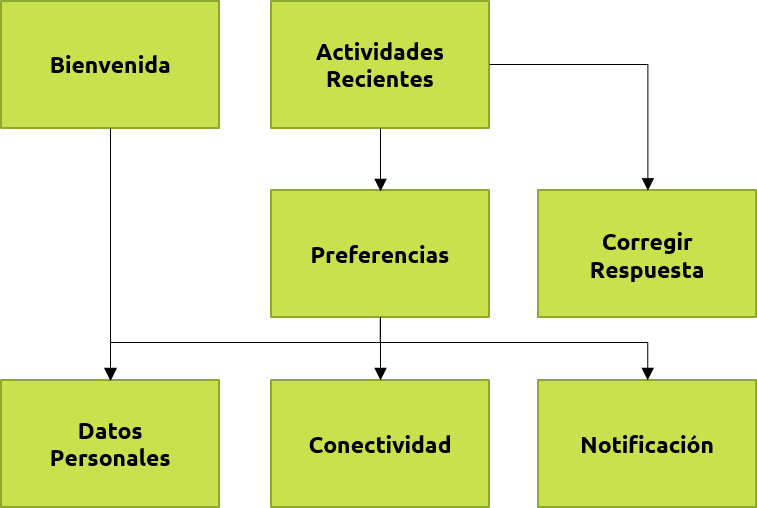
\includegraphics[width=0.7\columnwidth]{capitulo-5/graphics/navegacion}
\par\end{centering}
\caption[Mapa de navegación de pantallas de ActivitySurvey]{\label{fig5:navega}Mapa de navegación de pantallas de \emph{ActivitySurvey}}

\end{figure}

El diagrama de navegación de pantallas muestra la relación directa
entre pantallas por medio de cuadros y flechas. Una flecha que va
desde la pantalla \emph{Bienvenida} a otra pantalla \emph{Datos Personales}
ocurre por medio de una interacción del usuario en la pantalla \emph{Bienvenida}. 

\section{Resumen}

\label{sec56:conclusion}En este capítulo presentamos un servicio
de reconocimiento de actividades humanas (\abbr{HAR}) para la plataforma
\emph{\abbr{Android}}. Está construido en base a las mejores prácticas
de servicios utilitarios de implementación privada existentes como\emph{
Google Play Services}. Este utilitario permite que aplicaciones móviles
desarrolladas por terceros no dependan de implementaciones privativas
sino de un componente de software libre. Bajo un modelo colaborativo,
cualquier solución que utilice esta alternativa obtiene beneficios
como adaptarlo a sus necesidades o gozar de las mejoras evolutivas. 

Además, esta implementación fue probada por medio de una aplicación
móvil independiente donde se evaluó el funcionamiento desacoplado
proveído por el marco de trabajo de \emph{\abbr{Android}}. Los desarrollos
obtenidos han resultado satisfactorios desde el punto de vista de
su programación en lo que respecta a la integración entre implementaciones
de aplicación móvil y el servidor utilitario separados en procesos
independientes. En el siguiente capítulo se tratará de la recolección,
validación y análisis de información en terreno a través de la aplicación
de encuesta.
